\subsection{Dual simplex}

Instead of walking over the bfs of the primal LP we walk around the feasible solutions of the dual problem. This is sometimes useful for example if it's easy to find an initial dual solution. Later in the course we'll see an algorithm that adds constraints. Primal solutions may get infeasible by this. For the dual that doesn't matter.

See figure \ref{Fig:ballsOfSteel} for how dual solutions look like and figure \ref{Fig:dualSimplex} for a run of dual simplex.

\begin{figure}[hbt]
\begin{center}
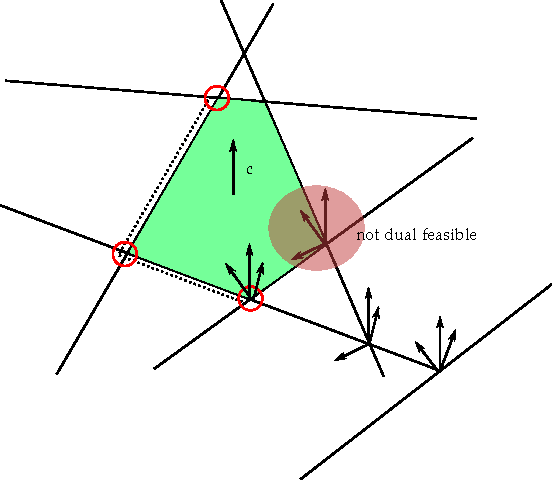
\includegraphics{./images/dualSimplex.pdf}
\end{center}
\caption{Dual Simplex}
\label{Fig:dualSimplex}
\end{figure}

We still keep a basis $B$ and $x_B=A_B^{-1}b$ but $x_B$ need not be positive anymore. Third we keep $\trans y=c_BA_B^{-1}$ and then we work towards a feasible primal solution. $\trans y$ should be feasible so 

\[\trans y A \leq c \quad 0 \leq c-c_BA_B^{-1}A \quad 0\leq \bar c\]

Assume we have a dual feasible basis $B$. Our tableau looks like this:

\begin{center}
\begin{tabular}{c|c}
$-c_Bx_B$ & $\bar c = c-c_BA_B^{-1}A$\\\hline
$x_B=A_B^{-1}b$ & $A_B^{-1}A$ 
\end{tabular}
\end{center}

We know $\bar c = c-c_BA_B^{-1}A \geq 0$. If $x_B$ is positive, we're done. Otherwise there is some $x_{b_i}$ that is negative. We now kick out that index and bring in another one. Since we want to keep the costs greater than 0 we want to add a positive multiple $\Theta > 0$ of row $x_{b_i}$ to the cost vector, because there is a 1 in column $x_{b_i}$. That means we need

\[\bar c_k + \Theta v_k \geq 0,\quad \forall k\]

Where $v_k$ is the entry in ($x_{b_i}, k$). This is of course only interesting if $v_k<0$. We then need 

\[ \Theta \leq \frac{\bar c_k}{|v_k|} \quad \forall k\]

So we look for a column $j$ such that $v_j<0$ and 

\[j = \argmin{i} \frac{c_i}{|v_i|}\]

It can of course happen that all $v_k$ are greater than zero. Then the dual is unbounded, which means that the primal is infeasible. For a proof suppose the primal is feasible

\[\exists x\geq 0: Ax=b\]

If we multiply both sides with the inverse of the basis matrix we get TODO.

\begin{lstlisting}
Dual-Simplex
keep B s.t. $\trans y = c_BA_B^{-1}$ is feasible
until $x_B = A_B^{-1}b \geq 0$
	pick $b_i \in B$ s.t. $x_{b_i} <0$
	let $x_{b_i},v_1, v_2 \ldots, v_n$ be the row in the tableau
	if $v_k \geq 0\ \forall k$
		return Infeasible
	find j s.t. $v_j<0$ and $\bar c_j/|v_j|$ is minimal
	B = $B\backslash b_i \cup j$
return B
\end{lstlisting}

As with primal simplex this algorithm can start to cycle for degenerate problems. To avoid cycling always choose the lexicographically smallest row and among lexicographically equal rows the one with the smallest index.

This algorithm can also be used to find an initial solution for the regular simplex algorithm. We can replace the cost vector by $0$ such that every feasible solution is optimal. We can then build the dual

\begin{align*}
\max \quad & \trans b y\\
s.t.\quad & \trans y A = 0\\
&y \text{ free}
\end{align*}